\chapter{Конструкторская часть}

В данном разделе будут рассмотрены требования к программе и
алгоритмы визуализации сцены и погодных явлений.

\section{Общий алгоритм визуализации \\трехмерной сцены}

Рассмотрим алгоритм визуализации сцены:
\begin{enumerate}[label=\arabic*)]
    \item Задать объекты сцены.
    \item Задать источник света.
    \item Используя $Z$-буфер получить изображение сцены.
    \item Отобразить тени, используя теневые карты, полученные с помощью \\$Z$-буфера.
    \item Изобразить молнию.
    \item Если идет дождь, то пока в буфере есть частицы осадков, выполнить:
    \begin{enumerate}[label=\arabic*)]
        \item Используя систему частиц, наложить осадки на изображение.
        \item Нарисовать изображение.
        \item Обновить буфер системы частиц.
    \end{enumerate} 
\end{enumerate} 

\section{Алгоритм $Z$-буфера}

На рисунках \ref{img:r1} -- \ref{img:r2} представлены схемы алгоритмов $Z$-буфера и модифицированного $Z$-буфера для теневых карт.

\begin{figure}[H]
	\centering
	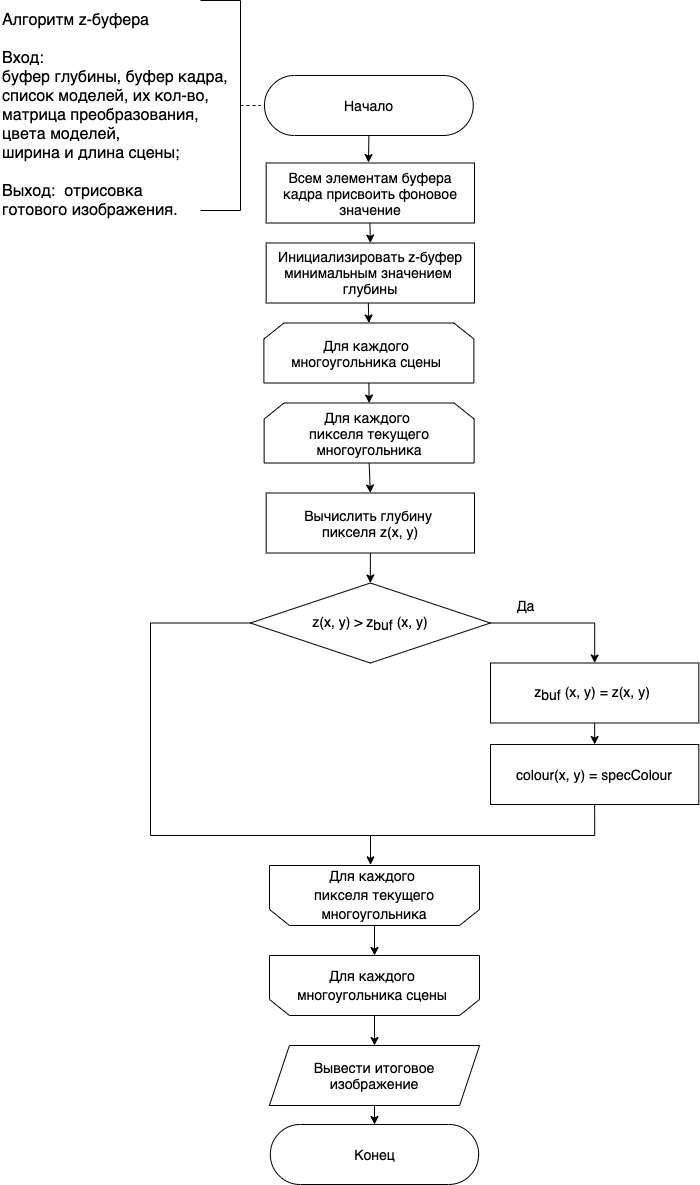
\includegraphics[scale=0.6]{include/zbuf.png}
	\caption{Алгоритм $Z$-буфера}
	\label{img:r1}
\end{figure} 

\begin{figure}[H]
	\centering
	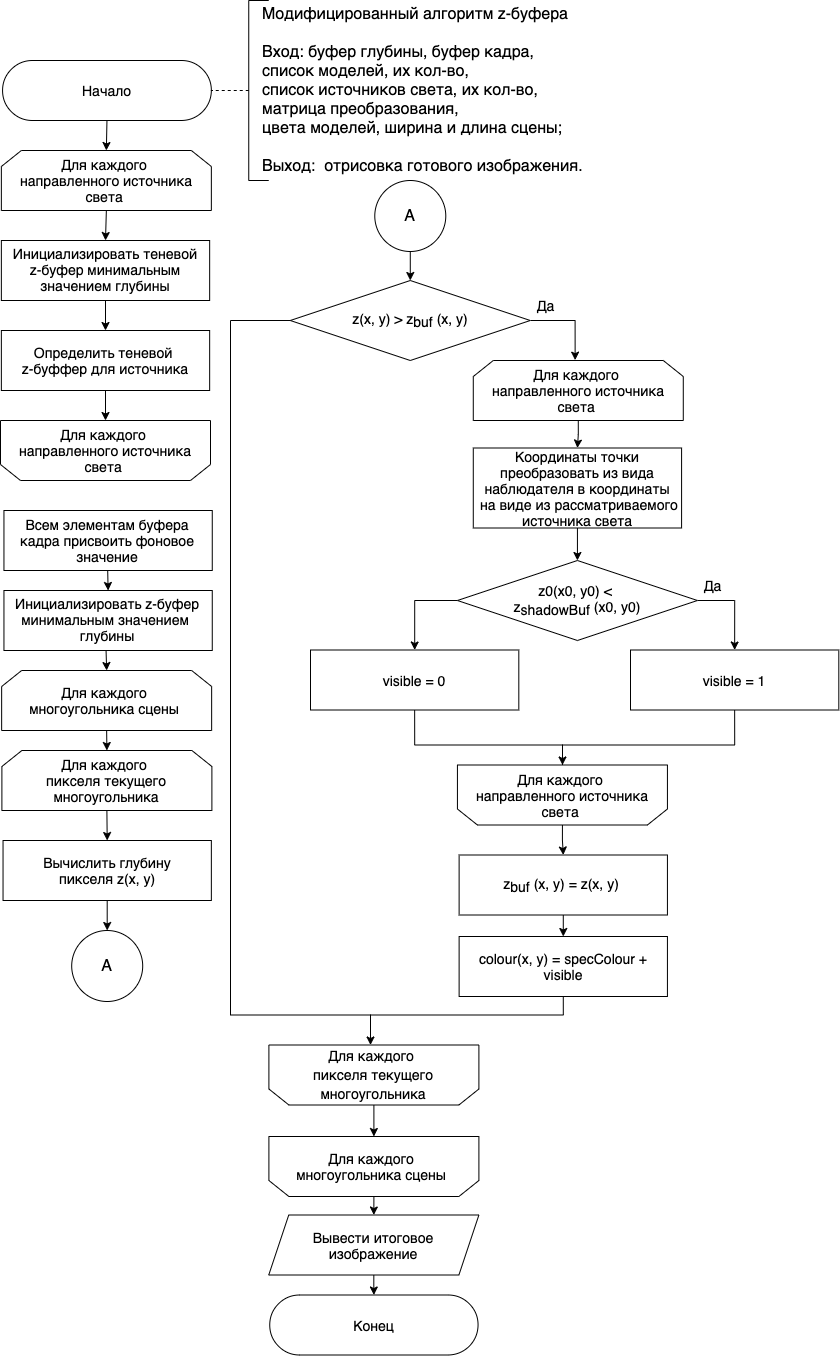
\includegraphics[scale=0.5]{include/mod_zbuf.png}
	\caption{Модифицированный алгоритма z-буфера}
	\label{img:r2}
\end{figure} 

\section{Алгоритм генерации молнии}

На рисунке \ref{img:lightning} представлена схема алгоритма генерации молнии.

\begin{table}[h!]
	\centering
	\begin{tabular}{p{1\linewidth}}
		\centering
		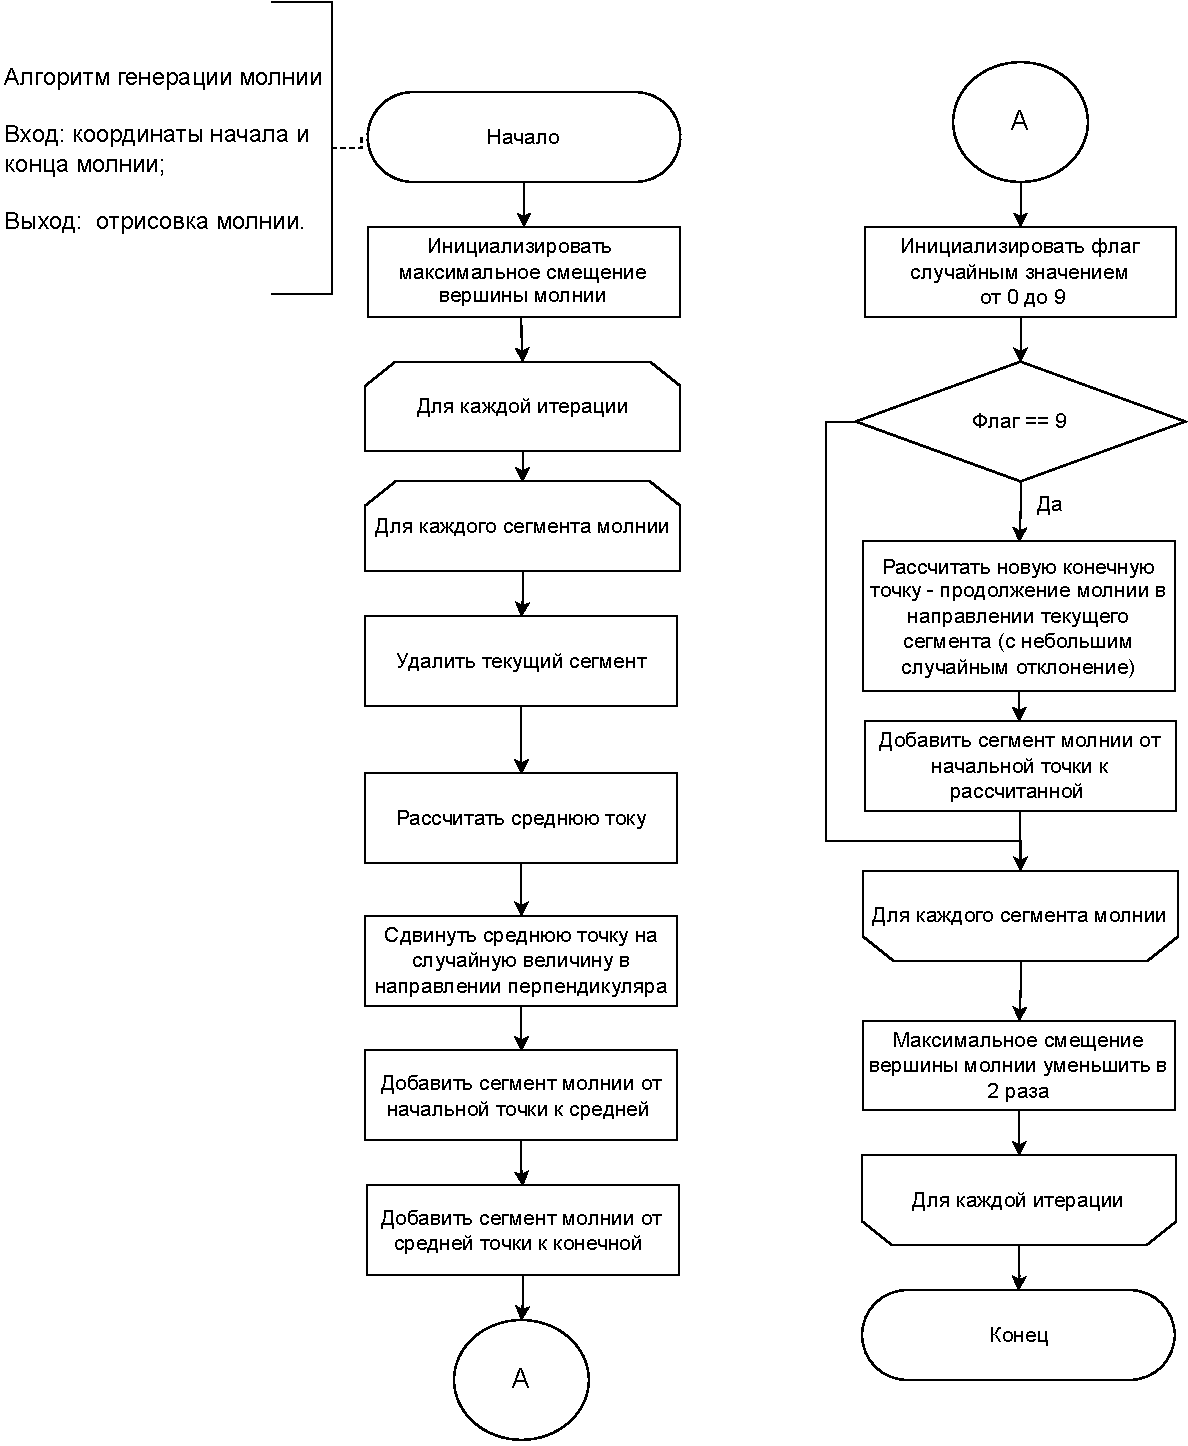
\includegraphics[width=0.88\linewidth]{include/lightning.pdf}
		\captionof{figure}{Схема алгоритма генерации молнии}
		\label{img:lightning}
	\end{tabular}
\end{table}
\newpage
На рисунке \ref{img:r4} представлена генерации молнии.

\begin{figure}[H]
	\centering
	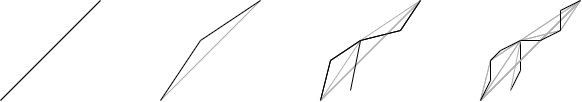
\includegraphics[scale=0.5]{include/lightning.png}
	\caption{Генерация молнии}
	\label{img:r4}
\end{figure} 

\section{Алгоритм генерации осадков}

На рисунке \ref{img:r3} представлена схема алгоритма генерации осадков.
\begin{figure}[H]
	\centering
	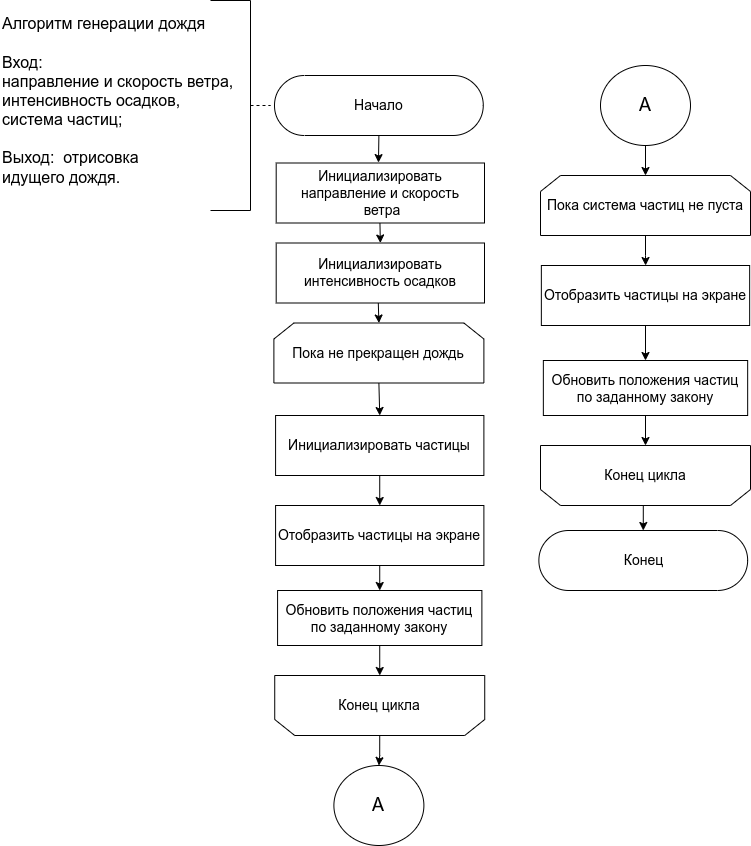
\includegraphics[scale=0.55]{include/rain.png}
	\caption{Алгоритм генерации осадков}
	\label{img:r3}
\end{figure} 

\section{Разработка и обоснование используемых типов и структур данных}

Для разрабатываемого ПО нужно будет реализовать следующие типы и
структуры данных.
\begin{enumerate}[label=\arabic*)]
	\item Структура сцены -- список объектов сцены, список источников света.
	\item Объекты сцены задаются массивом полигонов
        \item Полигоны содержат три точки, цвет полигона
	\item Цвет -- вектор из трех чисел (три целочисленные переменные, характерезующие цветовую модель $RGB$).
	\item Структура молнии содержит вектор, характеризующий главную и побочные ветви и содержащий точки изгибов.
	
	\item Структура системы частиц содержит в себе:
	\begin{itemize}
		\item Координаты положения частиц в пространстве.
		\item Направление их движения.
	\end{itemize}
	\item Структура источника света содержит:
	\begin{itemize}
		\item Координаты положения источника света в пространстве.
		\item Интенсивность излучения (вещественное число).
	\end{itemize}
\end{enumerate}

\section{Вывод}

В данном разделе были рассмотрены реализованные алгоритмы и описаны представления данных и используемых структур.